\documentclass[twocolumn]{article}

\usepackage[english]{babel}
\usepackage[a4paper,top=2cm,bottom=2cm,left=3cm,right=3cm,marginparwidth=1.75cm]{geometry}

% packages
\usepackage{amsmath}
\usepackage{graphicx}
\usepackage{xcolor}

% colors
\definecolor{BlueLUH}{cmyk}{1.0,0.7,0,0} 
\colorlet{linkcolor}{BlueLUH}
\usepackage[colorlinks=true, allcolors=linkcolor]{hyperref}

% information
\title{\LARGE \bf PerfTuner \\Developer Documentation}
\author{Thomas Gantz \and Alexander Goebel \and Soumili Samanta}
\date{March 20, 2024}

\begin{document}
\maketitle

\begin{abstract}
    The goal of the PerfTuner project is to exploit LLMs (in our case we use ChatGPT from OpenAI) to optimize C++ functions by using advanced vector extensions (AVX). AVX intrinsics are C++ functions that use single instruction multiple data (SIMD) functionalities included in AMD and Intel CPUs.  
    \begin{figure}[h]
        \centering
        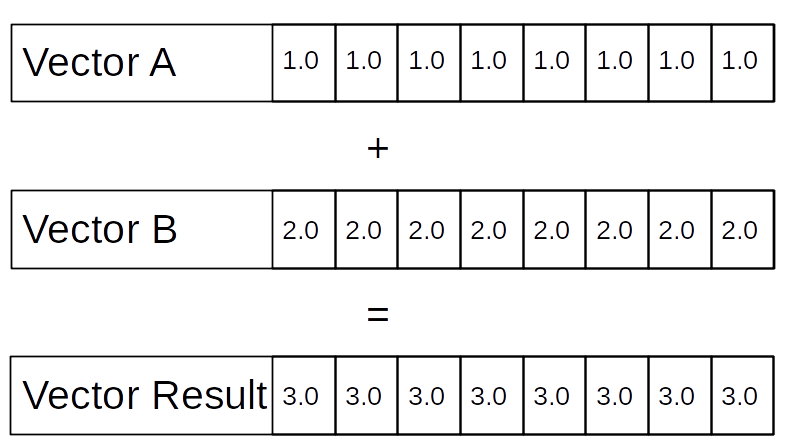
\includegraphics[width=0.4\textwidth]{images/AVX_principle.png} 
        \caption{Example for AVX. 8 floating point numbers can be added with a single instruction.}
        \label{fig:bild1}
    \end{figure}
\end{abstract}

\section{Introduction}
In this document we explain the main ideas of our implementation. In chapter \ref{structure} we describe the structure of our repository. The main program flow can be observed in chapter \ref{flow}. All important files are described in chapters \ref{files}, \ref{problems} and \ref{snippets}. In chapter \ref{experiences} we describe some of the experiences we made during the project and in chapter \ref{future} we suggest some possible steps for future improvements of this project.

\section{Repository} \label{structure}
The repository can be found under \url{https://github.com/pvs-hd-tea/23ws-PerfTuner}. The root directory consists of the two folders \textit{Product} and \textit{docs}. The folder \textit{Product} contains all software related files whereas the folder \textit{docs} contains the documentation, including this file.\\
\\
In \textit{Product} you can find all needed functions. They are explained in detail in chapter \ref{files}. 
Furthermore it contains the folders \textit{Problems} (\ref{problems}), \textit{Snippets} (\ref{snippets}) and \textit{Statistics}. All examples for the automatic evaluation (\ref{auto}) can be found in \textit{Problems}. Code snippets used for guiding the LLM are in the folder \textit{Snippets}. Finally \textit{Statistics} contains graphs from the automatic evaluation loop.

\section{Program Flow} \label{flow}
\begin{figure}[h]
    \centering
    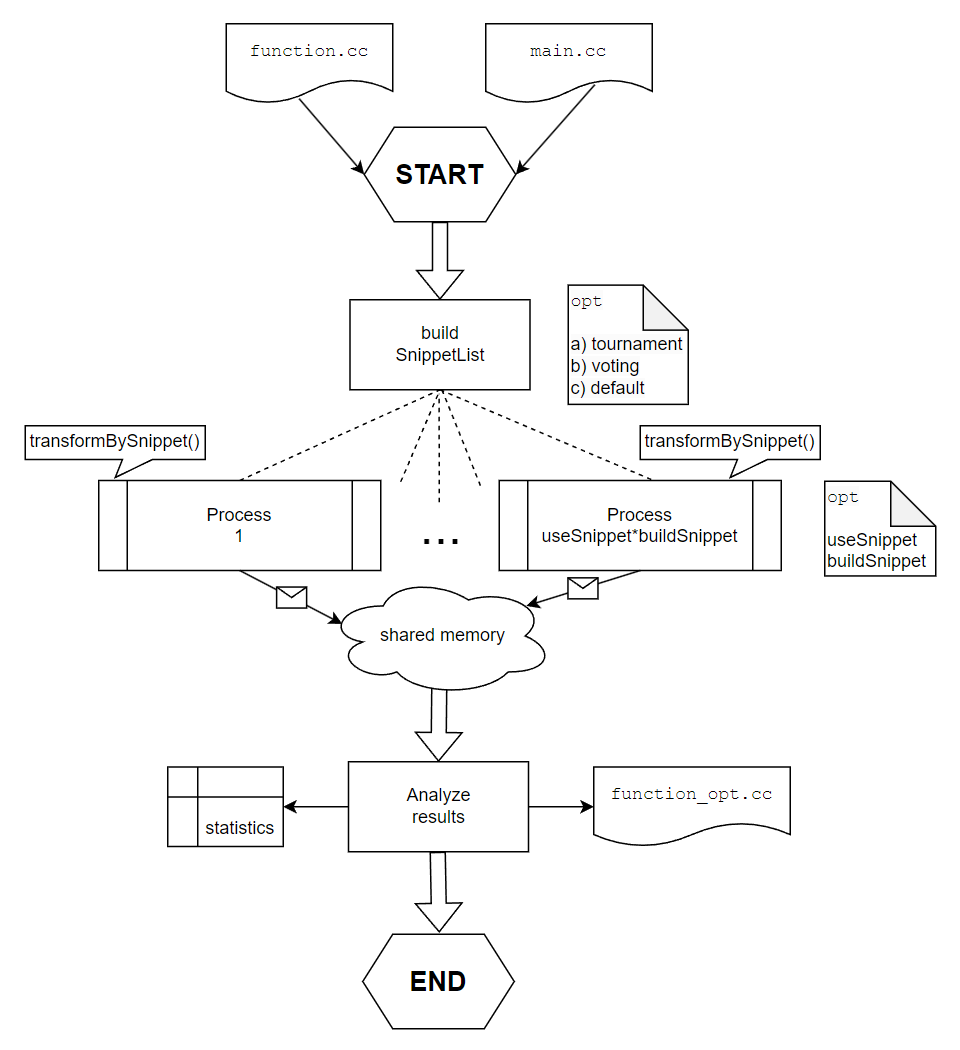
\includegraphics[width=0.5\textwidth]{images/architecture.png} 
    \caption{Flowchart illustrating the architecture}
    \label{fig:bild1}
\end{figure}

\section{Files} \label{files}
\subsection{perftuner}
This function is the entry point for the user. It can be called in a terminal by \textit{python3 perftuner.py}. The user is asked to supply the path of the relevant files, i.e. a file called \textit{function.cc} which contains the code to be optimized and a file called \textit{main.cc} containing the testing environment as explained in \ref{test}. The user is also asked how many snippets (see \ref{transform}) and how many attempts by the LLM should be tried for the optimization. Finally, he is asked to choose the method (voting (\ref{find}), tournament (\ref{findTournament}) or default) for finding the right snippet.

\subsection{PerfTunerClass}
\label{PerfTunerClass}
The \texttt{PerfTuner} class is the core of the program. In its constructor, the settings of a transformation are configured when a \texttt{PerfTuner} is instantiated, and the invocation of its \texttt{do} method initiates an actual transformation, returning its statistics in an array.\\ 
\\
It is crucial to specify the paths for locating the function to be transformed (\textit{function.cc}) and the testing environment (\textit{main.cc}). Additionally, the user can determine the methodology for constructing a \texttt{SnippetList} that ranks the snippets by relevance to the problem. Options include tournament, voting, or the default, where snippet 10 (LU decomposition) is selected, typically yielding optimal results for most problems, although an alternative can be specified. The user can also specify the number of snippets from the list to use in \texttt{runs\_useSnippet} and the frequency of attempts for each snippet in \texttt{runs\_buildSnippet}.\\
\\
Upon completion, the results of all processes are presented to the user, including the success rate per snippet and the \texttt{transformationQualityAverage}, which represents the averaged sum of the status of all transformations per snippet, serving as an index of the effectiveness of a snippet. Finally, the best \textit{function\_opt.cc} is copied to a readily accessible location for the user within the \texttt{PerfTuner} class.\\
\\
The \texttt{do} method initially constructs a \texttt{SnippetList} based on the specified settings and then executes \texttt{runs\_useSnippet * runs\_buildSnippet} transformation processes accordingly. It's noteworthy that each process generates its own output files. Communication occurs via the shared memory \texttt{jobsStatusArray}. Crucial information is conveyed through status codes, with the following interpretations:
\begin{itemize}
    \item \texttt{-99}: The process wasn't active
    \item \texttt{-4}: FAIL: \textit{function.cc} didn't compile
    \item \texttt{-3}: FAIL: \textit{function\_opt.cc} didn't compile
    \item \texttt{-2}: FAIL: The results are not identical
    \item \texttt{-1}: FAIL: \textit{function\_opt.cc} was slower
    \item \texttt{0}: SUCCESS
\end{itemize}

\subsection{transformBySnippet} \label{transform}
This function does the actual transformation and contains the main meta strategy of our approach. The parameters are the function to be optimized and a C++ snippet chosen by \ref{find}, \ref{findTournament} or a default snippet to speed up the process.\\
\\
As a first step the LLM is trained by the following mechanism: We ask the LLM to optimize the given snippet with AVX. However, we also directly supply the answer with a optimized version that we have written ourselves. We then ask the LLM to explain this optimization. By this trick we guide the LLM on how to transform the function in the last step.\\
\\
As a second and third step we use the LLM to identify all main sub tasks of the function and to determine which sub tasks can be optimized with AVX.\\
\\
In a final step we use the list of sub tasks and the guiding information of step one to optimize the function.\\
\\
Since the OpenAI API does not remember the last conversations we always have to supply the results of the former conversation. 

\subsection{AutomaticEvaluationLoop} \label{auto}
\texttt{AutomaticEvaluationLoop.py} aims to evaluate the product proficiencies and intricacies. It iterates over a set of predefined problem classes and their corresponding problems, attempting judge the results of producing optimized code. The process involves invoking the \texttt{\nameref{PerfTunerClass}} , which performs transformations and provides statistics on the optimization attempt.\\
\\
For each problem, collection and storing of appropriate parameters, and optimization statistics are done.\\
\\
\texttt{perftuner.do()} from \texttt{PerfTunerClass.py} stores all the statistical values required in list format.
These statistics help in producing the following tables and graphs:
\begin{itemize}
    \item \texttt{Table1}: Metrics determining problems solved in class-wise manner.
    \item \texttt{Table2}: Provides problem wise statistics.
    \item \texttt{Table3 Snippet success rate}: Provides percentage of times a particular snippet transformed orginal to optimized code.
    \item \texttt{Graph1 Solved status}: Provides graph determining problems solved and unsolved by our product.
    \item \texttt{Graph2 Speedup}: Provides bar graph representing execution time of original code and optimized code.
    \item \texttt{Graph3 Snippet chosen}: Provides a graph showing which snippet was chosen by which Problem.
\end{itemize}

\subsection{findSnippetList} \label{find}
The function \texttt{\nameref{transform}} requires a C++ code snippet closely related to \textit{function.cc}. For this purpose, we have compiled a snippet library (\ref{snippets}) containing various operations. This function is one of the methods for constructing the hierarchical \texttt{SnippetList}, employing a voting strategy to determine the most suitable snippet for the given function. Additionally, a crucial aspect of the function involves returning the \texttt{SnippetList} in a specific format, achieved by splitting the output string from ChatGPT in an array of strings (using a stack functionality) and subsequently employing pattern matching.

\subsection{findSnippetListByTournament} \label{findTournament}
Just like \ref{find} this function finds the best snippet suited for the given function. However, in contrast to the voting strategy a tournament strategy is used.
Two snippets of the library are taken at random and with the LLM it is determined which snippet is better suited for the given function. The winner is kept and the looser is discarded.\\ 
\\
This procedure is repeated in a tournament style. An overall winner, the runner up and the two remaining final 4 candidates are returned as as snippet list.

\subsection{test} \label{test}
This script is designed to assess the compilation and runtime performance of C++ code compared to its AVX-optimized version.\\ 
\\
It begins by compiling both the original C++ code and the AVX-optimized version using "g++". If either compilation fails, it returns an error code to signify the failure. 
Subsequently, it executes both compiled programs and measures their respective runtime using the `time` module. 
After execution, it compares the outputs of both programs. If there's a discrepancy between the outputs, it flags this as an issue.\\ 
\\
Throughout the process, the script handles platform differences by adjusting the commands for Windows and non-Windows environments accordingly.

\subsection{askChatGPT}
The \texttt{askChatGPT} function is designed to interact with the GPT-3.5 model from OpenAI, utilizing its chat completion capabilities. It takes input file names, an output file name, and a message as arguments.\\ 
\\
If input files are provided, it reads the content of each file and appends it to the prompt string. It then creates an instance of the OpenAI class and requests completions from the GPT-3.5 model using the provided message and the constructed prompt. After receiving a response from the model, it extracts the generated text and checks if an output file name is provided.It constructs the output file, writes the generated text to the file, and closes any opened input files.

\subsection{TaskCode}
This file contains the task code that is performed by every process instantiated in the \texttt{PerfTuner} class to do a transformation. The actual transformation is performed by \texttt{\nameref{transform}}. This is the wrapper for the transforming processes. Note the parameters \texttt{i} and \texttt{j} that identify a process and are essential for communication with the main process of the \texttt{PerfTuner} class over the shared memory \texttt{jobsStatusArray}. Also note the different file paths since every process has its own output files for its transformation.

\subsection{.env}
This file should contain a valid key (token) for using OpenAI. The format is: OPENAI\_API\_KEY=xxx where xxx is the corresponding key.

\section{Problems} \label{problems}
All examples for the automated evaluation are in the folder \textit{Problems}. They are divided into three classes of difficulty. For each example there is a sub folder containing the C++ files \textit{function.cc} and \textit{main.cc}. As described in \ref{test} \textit{function.cc} is the code that needs to be optimized and \textit{main.cc} contains the test environment. 

\section{Snippets} \label{snippets}
As described in \ref{transform} we use code snippets to guide the LLM in the optimization process. Currently we have 11 such snippets and the corresponding (by hand) optimized versions. The library contains all snippets. 

\section{Our Experiences} \label{experiences}
Throughout our project, we've explored various approaches and gained diverse experiences, with many proving unsuccessful.

\subsection{Plain ChatGPT}
Initially, we attempted to prompt immediate transformations by experimenting with different prompts, many of which were already highly technical or tailored to the specific problem. However, this approach seldom yielded satisfactory results. We've since learned that it's necessary to engage ChatGPT in a more nuanced manner, aiming to put it in the right mindset for productive interactions.

\subsection{Pseudo Code Strategy}
As a different meta strategy we ask the LLM to translate the C++ snippet and the function into pseudo code. Consequently, we asked to re translate the pseudo code into C++ code with AVX intrinsics. However, the results obtained by this approach were not useful and did not produce compilable code.  

\subsection{Using Google for Transformations}
The code was created in order to make transformation easier with the support of Google search. The code started by reading C++ code from a file named \textit{function.cc}. Then, it utilized OpenAI's ChatGPT to generate a concise Google search query based on the code's functionality. After performing a Google search and extracting relevant content, the script interacted with ChatGPT again to obtain AVX2 code snippets tailored for optimizing the C++ code. Once received, these snippets were integrated into a runnable program, which was then stored in files for further use. Overall, the script automated the process of optimizing C++ code using AI-driven understanding and web scraping techniques. However, the results did not match up to the benchmark by our current product. 

\subsection{Issues with OpenAI}
There's a possibility of exceeding the token limit per minute imposed by OpenAI during the transformation process, especially when utilizing multiple cores (though even with just 4 cores, it can occur). At times, OpenAI's response times were exceptionally slow, leading to no answers for several minutes. In such cases, the program may hang indefinitely. Another issue we've encountered is the inconsistency in the output format. For instance, requesting a list may result in formats like "1. 2. 3." or "- - -". While we've addressed this by crafting prompts that usually yield the desired output, we've also implemented a "while true-try" approach to catch instances where the desired format isn't achieved.

\section{Future Steps} \label{future}
If the project is continued, we would suggest the following steps:
\begin{enumerate}
    \item Transform whole programs.
    \item Speed-up: multiprocessing (in particular for finding the snippet).
    \item Expand the library (use floats, doubles and integers; more complex problems, e.g. for Fourier Transformation).
    \item Experiment with different prompts.
    \item Use user feedback and snippets to improve the results (open the possibility for the user to supply a snippet).
    \item Generate a \textit{main.cc} automatically.
    \item Train the model with the snippets (model fine-tuning).
    \item Try more coding specific LLMs.
    \item Implement iterative refinement (if there is a working result: make it even better).
\end{enumerate}

\end{document}